\documentclass[a4paper, 11pt]{book}
\usepackage{anyfontsize}
\usepackage[CJKchecksingle, AutoFakeBold]{xeCJK}
\usepackage{CJKnumb}

\usepackage{setspace}
\onehalfspacing
\renewcommand{\arraystretch}{1}

\setlength{\parindent}{2em}

\usepackage[intlimits, leqno]{amsmath}
\usepackage{amsthm}
\usepackage{amssymb}

\usepackage{fontspec}
\usepackage{unicode-math}

\setmainfont[
    Extension=.otf,
    UprightFont=*-Regular,
    BoldFont=*-Bold,
    ItalicFont=*-Italic,
    BoldItalicFont=*-BoldItalic
]{STIXTwoText}

\setmathfont[
    Extension=.otf,
    BoldFont=*
]{STIXTwoMath-Regular}

\let\exerciseQuestion\Question
\AtBeginDocument{%
    \let\mathQuestion\Question
    \let\Question\exerciseQuestion
}

\setsansfont{TeX Gyre Heros}
\setmonofont{Courier New}

\usepackage{esint}

\DeclareSymbolFont{CMlargesymbols}{OMX}{cmex}{m}{n}
\let\sumop\relax\let\prodop\relax
\DeclareMathSymbol{\sumop}{\mathop}{CMlargesymbols}{"50}
\DeclareMathSymbol{\prodop}{\mathop}{CMlargesymbols}{"51}

\usepackage{euscript}

\newcommand{\bm}{\symbfit}
\newcommand{\smalltriangle}{\mathbin{\vcenter{\hbox{\scalebox{0.65}{$\triangle$}}}}}

\setCJKmainfont[
    ItalicFont=FZKai-Z03S
]{FZShuSong-Z01S}

\setCJKsansfont[
    BoldFont=* Medium,
    ItalicFont=FZKai-Z03S
]{Noto Sans CJK SC}

\setCJKmonofont[
    ItalicFont=FZKai-Z03S
]{FZShuSong-Z01S}

\setCJKfamilyfont{kai}{FZKai-Z03S}

\setCJKfamilyfont{song}[
    ItalicFont=FZKai-Z03S
]{FZShuSong-Z01S}

\setCJKfamilyfont{fangsong}[
    ItalicFont=FZKai-Z03S
]{FZFangSong-Z02S}

\setCJKfamilyfont{hei}{Noto Sans CJK SC Medium}
\setCJKfamilyfont{hei2}[
    BoldFont=* Bold
]{Noto Sans CJK SC}

\setCJKfamilyfont{black}[
    BoldFont=* Black
]{Noto Sans CJK SC}

\setCJKfamilyfont{sectionfont}[
    BoldFont=* Black
]{Noto Sans CJK SC}

\setCJKfamilyfont{pffont}[
    BoldFont=* Medium
]{Noto Sans CJK SC}

\setCJKfamilyfont{emfont}[
    BoldFont=* Medium
]{Noto Sans CJK SC}

\defaultfontfeatures{Ligatures=TeX} 
\XeTeXlinebreaklocale "zh"
\XeTeXlinebreakskip=0pt plus 1pt minus 0.1pt

\newcommand\kaishu{\CJKfamily{kai}}
\newcommand\songti{\CJKfamily{song}}
\newcommand\heiti{\CJKfamily{hei}}
\newcommand\thmheiti{\CJKfamily{hei2}}
\newcommand\fangsong{\CJKfamily{fangsong}}
\renewcommand{\em}{\bfseries\CJKfamily{emfont}}


\usepackage[unicode, colorlinks]{hyperref}
\hypersetup{
	linkcolor=blue,
	citecolor=red,
	urlcolor=teal,
	pdfauthor={王畅},
	pdftitle={ICS 问题求解(2021 秋)}
}

\usepackage[iso, english]{isodate}
\usepackage{geometry}
\geometry{
	paper=a4paper,
	top=3cm,
	inner=2.54cm,
	outer=2.54cm,
	bottom=3cm,
	headheight=6ex,
	headsep=6ex,
}

\usepackage[dvipsnames]{xcolor}

\usepackage{paralist}
\usepackage{commands}
\usepackage[figurewithin=none]{caption}
\usepackage{graphicx}
\usepackage{float}
\usepackage{tikz}
\usetikzlibrary{shapes.symbols, backgrounds, matrix, calc, arrows, math, arrows.meta}
\usepackage{minted}

\numberwithin{equation}{chapter}
\renewcommand{\theequation}{\thechapter.\arabic{equation}}

\usepackage{datetime}

\usepackage{xstring}
\usepackage{fancyhdr}
\newcommand\sectionname{\arabic{chapter}.\arabic{section}}
\pagestyle{fancy}
\renewcommand{\chaptermark}[1]{\markboth{
	第\CJKnumber{\thechapter}周\quad #1
	}{}}
\renewcommand{\sectionmark}[1]{\markright{\arabic{chapter} \quad #1}}
\fancyhf{}
\fancyhead[EC]{\CJKfamily{hei2}\footnotesize{\leftmark}\vspace{1mm}}
\fancyhead[OC]{\CJKfamily{hei2}\footnotesize{\rightmark}\vspace{1mm}}
\fancyhead[LE, RO]{{\footnotesize \thepage}\vspace{1mm}}
\fancyhead[RE, LO]{}
\renewcommand{\headrulewidth}{0.5pt}
\renewcommand{\footrulewidth}{0pt}
\addtolength{\headheight}{0.5pt}

\fancypagestyle{plain}{%
	\fancyhead{}
	\renewcommand{\headrulewidth}{0pt}
}

\usepackage[many]{tcolorbox}

\newtcolorbox{summary}{
	breakable,
	enhanced,
	width=\textwidth,
	colback=white, colbacktitle=white,
	colframe=gray!50, boxrule=0.2mm,
	coltitle=black,
	fonttitle=\bfseries\sffamily,
	attach boxed title to top left={yshift=-\tcboxedtitleheight/2, xshift=\tcboxedtitlewidth/4},
	boxed title style={boxrule=0pt, colframe=white},
	after skip=1cm,
	top=3mm,
	bottom=3mm,
	title={要点}
}

\usepackage[calcwidth, explicit, nobottomtitles, newparttoc, indentafter]{titlesec}
\usepackage{titletoc}
\usepackage[titles]{tocloft}
\cftsetpnumwidth{1.75em}
\providecommand{\dmchapterttl}[1]{\IfSubStr{ABCDEFGHIJKLMNOPQRSTUVWXYZ}{#1}{附录 #1	}{第\CJKnumber{#1}周}}

\newlength{\BoxTtlwidth}

\newcommand{\MakeChapBox}[2]{%
	\settowidth{\BoxTtlwidth}{\dmchapterttl{#1}}
	\begin{tcolorbox}[
		enhanced jigsaw,
		skin=bicolor,
		frame engine=path,
		sharp corners=all,
		width=0.9\textwidth,
		top=4mm, bottom=4mm,
		sidebyside,
		frame hidden,
		boxrule=0mm,
		lefthand width=\BoxTtlwidth,
		colupper=white,
		colback=gray!80,
		colbacklower=gray!10,
		sidebyside align=center,
		halign=center]
		\dmchapterttl{#1}
		\tcblower
		#2
	\end{tcolorbox}%
}

\newcommand{\MakeChapBoxSingle}[1]{%
	\begin{tcolorbox}[
		enhanced,
		width=0.7\textwidth,
		sharp corners=all,
		top=4mm, bottom=4mm,
		frame hidden,
		boxrule=0mm,
		colback=gray!10,
		halign=center]
		#1
	\end{tcolorbox}
}

\newtcbox{\MakeSectBox}{
	enhanced,
	arc=0pt, outer arc=0pt,
	before skip=0pt, after skip=0.4em, left skip=0pt, right skip=0pt,
	top=0pt, left=0pt, right=0pt, bottom=1.5mm,
	sharp corners=all,
	valign=bottom,
	colback=white,
	colframe=white,
	boxsep=0pt, leftrule=0pt, rightrule=0pt, toprule=0pt, bottomrule=0pt,
	overlay={ \draw[line width=1pt] (interior.south west) -- (interior.south east); }
}

\titleformat{name=\chapter}
	{\filright\sffamily\CJKfamily{black}\bfseries\Huge}
	{}
	{0mm}
	{\MakeChapBox{\thechapter}{#1}}
	[]
\titlespacing*{name=\chapter}
	{1pc}{*4}{1em}

\titleformat{name=\chapter, numberless}
	{\filcenter\sffamily\CJKfamily{black}\bfseries\Huge}
	{}
	{0mm}
	{\MakeChapBoxSingle{#1}}
	[{\if@mainmatter
		\addcontentsline{toc}{chapter}{#1}
		\markboth{#1}{}
	\fi}]
\titlespacing*{name=\chapter, numberless}
	{1pc}{*4}{1em}

\titleformat{name=\section}
	{\filleft\normalfont\sffamily\bfseries\CJKfamily{sectionfont}}
	{}
	{0mm}
	{ \settowidth{\BoxTtlwidth}{\Huge \thesection \hspace{0.7em} \Large #1}
		\ifdim \BoxTtlwidth < \textwidth
			\MakeSectBox{\Huge \thesection \hspace{0.7em} \Large #1}\vskip-18pt%
		\else
			\Huge \underline{\thesection} \hspace{0.7em} \Large #1%
		\fi%
	}
	[]

\titleformat{name=\section, numberless}
	{\filleft\normalfont\sffamily\bfseries\CJKfamily{sectionfont}}
	{}
	{0mm}
	{ \settowidth{\BoxTtlwidth}{\Large #1}
		\ifdim \BoxTtlwidth < \textwidth
			\MakeSectBox{\Large #1}\vskip-18pt%
		\else
			\Large #1
		\fi
	}
	[]
	
\titlespacing*{name=\section}
	{1pc}{*1.3}{*1}

\usepackage{zhnumber}
\usepackage[answerdelayed, lastexercise]{exercise}
\renewcommand{\ExerciseListName}{}
\renewcommand{\AnswerListName}{}
\renewcommand{\ExerciseHeaderNB}{\theExercise}
\renewcommand{\QuestionNB}{(\arabic{Question})}
\renewcommand{\ExerciseHeaderOrigin}{\ ({\kaishu\ExerciseOrigin})}
\renewcommand{\ExerciseListHeader}{\ExerciseHeaderDifficulty\textbf{\ExerciseHeaderNB}\ExerciseHeaderOrigin\textbf{.}\enspace}
\renewcommand{\AnswerListHeader}{\textbf{\ExerciseHeaderNB.}\enspace}
\renewcounter{Exercise}[chapter]
\renewcommand{\AtBeginAnswer}{\vspace{-1\baselineskip}}
\newcommand{\pro}{\Exercise}
\newcommand{\qn}{\Question}
\newcommand{\subqn}{\subQuestion}
\newcommand{\sol}{\Answer}

\makeatletter
\renewcommand{\@@@ExeCmd}{%
	\ifnum\@QuestionLevel=0
		\advance \@QuestionLevel by 1
		\begin{list}{\@getExerciseInfo\ExerciseListHeader}%
		{\partopsep \Exepartopsep \labelsep \Exelabelsep \itemsep \Exesep \listparindent 2em%
		\parsep \Exeparsep \topsep \Exetopsep \labelwidth \Exelabelwidth%
		\leftmargin \Exeleftmargin \rightmargin \Exerightmargin}
	\else
		\termineliste{1}\@EndExeBox
	\fi
	\@selectExercise
	\global\@Answerfalse\@BeginExeBox\refstepExecounter%
	\addcontentsline{\ext@exercise}{\toc@exercise}{\ExerciseName\
	\theExercise\ \expandafter{\itshape \ExerciseTitle}\hspace{.66em}}
	\item\ignorespaces\AtBeginExercise
}
\makeatother

\newcounter{soleq}
\counterwithin{soleq}{chapter}
\newenvironment{soleq}{\refstepcounter{soleq}\equation}{\tag{S-\thesoleq}\endequation}

\makeatletter
\newenvironment{problems}{%
	\begin{ExerciseList}
		\global\setbox\temp@Answerbox%
		\vbox{\unvbox\all@Answerbox\section*{第\zhnum{chapter}周}\unvbox\@Exercisebox\vskip\z@}%
		\global\setbox\all@Answerbox\copy\temp@Answerbox
		}{
	\end{ExerciseList}
}

\newenvironment{choices}{\begin{compactenum}[\quad\ \,A.{\ \ \ }]}{\end{compactenum}}

\newenvironment{hint}{%
	\ifvmode
		\ignorespaces
	\else
		\quad
	\fi
	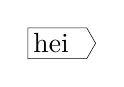
\begin{tikzpicture}[baseline=(H.base), every node/.style={signal, draw, very thin, signal to=east, signal from=nowhere, signal pointer angle=120, inner sep=2pt}]
		\node[anchor=mid west] (H) at (0,0) {\heiti\footnotesize 提示};
	\end{tikzpicture}
}{}

\g@addto@macro\frontmatter{\setcounter{tocdepth}{1}
	\setcounter{page}{1}
	\thispagestyle{empty}
	\addtocontents{toc}{\protect\thispagestyle{empty}}
	
	\renewcommand{\contentsname}{目录}
	\tableofcontents
}

\renewcommand{\figurename}{图}
\renewcommand{\tablename}{表}

\renewcommand{\listfigurename}{图片索引}
\renewcommand{\listtablename}{表格索引}

\pretocmd{\listoffigures}{%
	\cleardoublepage
	\phantomsection
	\addcontentsline{toc}{chapter}{\listfigurename}
}{}{}
\pretocmd{\listoftables}{%
	\cleardoublepage
	\phantomsection
	\addcontentsline{toc}{chapter}{\listtablename}
}{}{}

\begin{document}
	\begin{titlepage}
		\vspace*{\stretch{1}}
		\noindent\begin{center}\rule{\linewidth}{2pt}\end{center}
		\vspace{0.5em}
		\begin{center}
			{\fontsize{32}{32} \selectfont \bfseries \sffamily \CJKfamily{sectionfont} ICS 问题求解} \\ \vspace{1.5em}
			\LARGE PKU 04832363:计算机系统导论讨论班
		\end{center}
		\noindent\begin{center}\rule{\linewidth}{2pt}\end{center}
		\vspace{1em}
		\begin{center}
			{\Large 2021 年秋} \\ \vspace{1em}
			{\Large 北京大学} \\ \vspace{1.5em}
		\end{center}
		\vfill
		\begin{center} \href{https://www.pku.edu.cn/}{
\includegraphics[height=64pt]{logo.eps}} \end{center}
	\end{titlepage}
	
	\newpage
	\thispagestyle{empty}
	\begin{center}
		\Large 编译于 {\today} \currenttime
	\end{center}
	\vfill
	\begin{flushleft}
		\large
    	\textbf{汇编:}王畅 \\
    	\textbf{勘误:}请写信到 \href{mailto:wchang@pku.edu.cn}{\texttt{wchang@pku.edu.cn}} \\
		编者仅做了汇编和微小的改动,主要内容均来源于往年计算机系统导论课程,请悉知。
    \end{flushleft}

	\frontmatter

	\mainmatter
	\chapter{位级表示}
	\begin{summary}
		\begin{compactitem}
			\item 知道整数、浮点数在系统的存储方式(字节序)。
			\item 熟练掌握整数、浮点数的位级表示规则,快速完成其同十进制数的相互转换。
			\item 理解整数、浮点数规范中的各类特殊数的计算方法及其性质。
			\item 运用浮点数舍入的规则进行运算,知道类型转换的基本规则,能针对整数、浮点数的一些常见“反常情况”进行判断。
		\end{compactitem}
	\end{summary}

	\begin{problems}
		\pro 在 x86-64 机器上,定义 \texttt{unsigned int A = 0x123456}。请画出 \texttt{A} 在内存中的存储方式:
		\begin{table}[H]
			\centering
			\begin{tabular}{|c|c|c|c|c|c|c|c|}
				\hline
				... & 低地址 & \multicolumn{4}{c|}{\texttt{A}} & 高地址 & ... \\ \hline
				\multicolumn{2}{|c|}{...} & {\qquad \qquad} & {\qquad \qquad} & {\qquad \qquad} & {\qquad \qquad} & \multicolumn{2}{c|}{...} \\ \hline
			\end{tabular}
		\end{table}
		定义 \texttt{unsigned short B[2] = \{0x1234, 0x5678\}}。请画出 \texttt{B} 在内存中的存储方式:
		\begin{table}[H]
			\centering
			\begin{tabular}{|c|c|c|c|c|c|c|c|}
				\hline
				... & 低地址 & \multicolumn{4}{c|}{\texttt{B}} & 高地址 & ... \\ \hline
				\multicolumn{2}{|c|}{...} & {\qquad \qquad} & {\qquad \qquad} & {\qquad \qquad} & {\qquad \qquad} & \multicolumn{2}{c|}{...} \\ \hline
			\end{tabular}
		\end{table}
		\pro 在 x86-64 机器上,有下列 C 代码:
		\begin{minted}[frame=single, fontsize=\small]{c}
    int main() {
        unsigned int A = 0x11112222;
        unsigned int B = 0x33336666;
        void *x = (void *)&A;
        void *y = 2 + (void *)&B;
        unsigned short P = *(unsigned short *)x;
        unsigned short Q = *(unsigned short *)y;
        printf("0x%04x", P + Q);
        return 0;
    }
		\end{minted}
		运行该代码,结果是什么?
		\pro 在 x86-64 机器上,有下列 C 代码:
		\begin{minted}[frame=single, fontsize=\small]{c}
    int main() {
        char A[12] = "11224455";
        char B[12] = "11445577";
        void *x = (void *)&A;
        void *y = 2 + (void *)&B;
        unsigned short P = *(unsigned short *)x;
        unsigned short Q = *(unsigned short *)y;
        printf("0x%04x", Q - P);
        return 0;
    }
		\end{minted}
		运行该代码,结果是什么?
		\pro 在 x86-64 机器上,有如下的定义:
		\begin{minted}[frame=single, fontsize=\small]{c}
    int x = ...; // 表达式 A
    int y = ...; // 表达式 B
    unsigned int ux = x;
    unsigned int uy = y;
		\end{minted}
		判断下表中的表达式是否等价:
		\begin{table}[H]
			\centering
			\begin{tabular}{|c|c|c|}
				\hline
				序号 & 表达式 \verb|A| & 表达式 \verb|B| \\ \hline
				1 & \verb|x > y| & \verb|ux > uy| \\ \hline
				2 & \verb+(x > 0) || (x < ux)+ & \verb|1| \\ \hline
				3 & \verb|x ^ y ^ x ^ y ^ x| & \verb|x| \\ \hline
				4 & \verb|((x >> 1) << 1) <= x| & \verb|1| \\ \hline
				5 & \verb|((x / 2) * 2) <= x| & \verb|1| \\ \hline
				6 & \verb|x ^ y ^ (~x) - y| & \verb|y ^ x ^ (~y) - x| \\ \hline
				7 & \verb|(x == 1) && (ux - 2 < 2)| & \verb|(x == 1) && ((!!ux) - 2 < 2)| \\ \hline
			\end{tabular}
		\end{table}
		\begin{hint}
			减法的运算优先级比按位异或高。布尔运算的结果都是有符号数。
		\end{hint}
		\pro 下列代码的目的是将字符串 \texttt{A} 的内容复制到字符串 \texttt{B},覆盖 \texttt{B} 原有的内容,并输出“Hello World”;但实际运行输出是“Buggy Codes”。尝试找到代码中的错误。
		\begin{minted}[frame=single, fontsize=\small]{c}
    int main() {
        char A[12] = "Hello World";
        char B[12] = "Buggy Codes";
        int pos;
        for (pos = 0; pos - sizeof(B) < 0; pos++)
            B[pos] = A[pos];
        printf("%s\n", B);
    }
		\end{minted}
		\pro 假设某浮点数格式为 1 位符号、3 位阶码、4 位小数。下表给出了用该格式表达的浮点数 $(-1)^SM \cdot 2^E$ 与其二进制表示的关系。完成下表。
		\begin{table}[H]
			\centering
			\begin{tabular}{|c|c|c|c|c|}
				\hline
				描述 & 二进制表示 & $M$(写成分数) & $E$ & $f$ \\ \hline
				负零 &  & / & / & \texttt{-0.0} \\ \hline
				/ & \verb|01000101| &  &  &  \\ \hline
				最小的非规格化负数 &  &  &  &  \\ \hline
				最大的规格化正数 &  &  &  &  \\ \hline
				一 &  &  &  & \texttt{1.0} \\ \hline
				/ &  &  &  & \texttt{5.5} \\ \hline
				$+\infty$ &  & / & / & / \\ \hline
			\end{tabular}
		\end{table}
		\pro 假设浮点数格式 A 为 1 位符号、3 位阶码、4 位小数,浮点数格式 B 为 1 位符号、4 位阶码、3 位小数。回答下列问题。
			\qn 格式 A 中有多少个二进制表示对应于正无穷大?
			\qn 考虑能精确表示的实数的最大绝对值。A 比 B 大还是比 B 小,还是两者一样?
			\qn 考虑能精确表示的实数的最小非零绝对值。A 比 B 大还是比 B 小,还是两者一样?
			\qn 考虑能精确表示的实数的个数。A 比 B 多还是比 B 少,还是两者一样?
		\pro 判断下列说法的正确性。
			\qn 对于任意的单精度浮点数 \texttt{a} 和 \texttt{b},如果 \texttt{a > b},那么 \texttt{a + 1 > b}。
			\qn 对于任意的单精度浮点数 \texttt{a} 和 \texttt{b},如果 \texttt{a > b},那么 \texttt{a + b > b + b}。
			\qn 对于任意的单精度浮点数 \texttt{a} 和 \texttt{b},如果 \texttt{a > b},那么 \texttt{a + 1 > b + 1}。
			\qn 对于任意的双精度浮点数 \texttt{d},如果 \texttt{d < 0},那么 \texttt{d * d > 0}。
			\qn 对于任意的双精度浮点数 \texttt{d},如果 \texttt{d < 0},那么 \texttt{d * 2 < 0}。
			\qn 对于任意的双精度浮点数 \texttt{d},\texttt{d == d}。
			\qn 将 \texttt{float} 转换成 \texttt{int} 时,既有可能造成舍入,又有可能造成溢出。
		\pro 遵循 IEEE 754 浮点数标准,考虑下列代码:
		\begin{minted}[frame=single, fontsize=\small]{c}
    for (int x = 0; ; x++) {
        float f = x;
        if (x != (int)f) {
            printf("%d", x);
            break;
        }
    }
		\end{minted}
		试问代码的运行结果是什么?或者死循环?
		\pro 遵循 IEEE 754 浮点数标准,考虑下列代码:
		\begin{minted}[frame=single, fontsize=\small]{c}
    int x = 33554466; // 2^25 + 34
    int y = x + 8;
    for ( ; x < y; x++) {
        float f = x;
        printf("%d ", x - (int)f);
    }
		\end{minted}
		写出程序的运行结果。
	\end{problems}

\chapter{位级表示{---}往年考题}
	\begin{problems}
		\proy{2018} 下列哪种类型转换既可能导致溢出,又可能导致舍入?
		\begin{choices}
			\item \texttt{int} 转 \texttt{float}
			\item \texttt{float} 转 \texttt{int}
			\item \texttt{int} 转 \texttt{double}
			\item \texttt{float} 转 \texttt{double}
		\end{choices}
		\proy{2018} 在采用小端法存储机器上运行下面的代码,输出的结果是?(\texttt{int}、\texttt{unsigned} 为 32 位长,\texttt{short} 为 16 位长,0\textasciitilde9 的 ASCII 码是 \texttt{0x30}\textasciitilde\texttt{0x39})
		\begin{minted}[frame=single, fontsize=\small]{c}
    char *s = "2018";
    int *p1 = (int *)s;
    short s1 = (*p1) >> 12;
    unsigned u1 = (unsigned) s1;
    printf("0x%x\n", u1);
		\end{minted}
		\begin{choices}
			\item \texttt{0x00002303}
			\item \texttt{0x00032303}
			\item \texttt{0xffff8313}
			\item \texttt{0x00008313}
		\end{choices}
		\proy{2018} 考虑如下函数
		\begin{minted}[frame=single, fontsize=\small]{c}
    void XOR(int x, int y) {
        y = x ^ y;
        x = x ^ y;
        y = x ^ y;
        printf(x, y);
    }
		\end{minted}
		则 $\texttt{XOR}(a, b)$ 的输出结果是什么?
		\begin{choices}
			\item $a, b$
			\item $b, a$
			\item $b, 0$
			\item $b, a\ \verb|^|\ b$
		\end{choices}
		\proy{2017} 假定一个特殊设计的计算机,将 \texttt{int} 型数据的长度从 4 字节 扩展为 $4N$ 字节,采用大端法。现将该 \texttt{int} 型所能表示的最小负数写入内存中,如下图所示。其中每个小矩形代表一个字节,请问 X 位置这个字节中的值是多少?
		\begin{figure}[H]
			\centering
			\MemoryLayout{%
				8/white/\relax,
				24/gray!25/{$4N$ 字节},
				32/white/\relax
			}{%
				\draw[thick] (0,0) -- ++(0,3) node[above] {低地址};
				\draw[thick] (-32,0) -- ++(0,3) node[above] {高地址};
				\draw[-{Stealth[angle'=45]}, thick] (-8.5,1) -- ++(0,3) node[above] {X};
			}
		\end{figure}
		\begin{choices}
			\item \texttt{00000000}
			\item \texttt{01111111}
			\item \texttt{10000000}
			\item \texttt{11111111}
		\end{choices}
		\proy{2017} 以下说法正确的是:
		\begin{choices}
			\item 负数加上负数结果都为负数
			\item 正数加上正数结果都为正数
			\item 用 \verb|&| 和 \verb|~| 可以表示所有的逻辑与或非操作
			\item 用 \verb|&| 和 \verb+|+ 可以表示所有的逻辑与或非操作
		\end{choices}
		\proy{2017, 2016} 若我们采用基于 IEEE 浮点格式的浮点数表示方法,阶码字段(exp)占据 $k$ 位,小数字段(frac)占据 $n$ 位,则最小的规格化正数是:
		\begin{choices}
			\item $(1-2^{-n}) \cdot 2^{-2^{k-1}+2}$
			\item $2^{-2^{k-1}+2}$
			\item $2^{-n} \cdot 2^{-2^{k-1}+2}$
			\item $(1-2^{-n}) \cdot 2^{-2^k+1}$
		\end{choices}
		\proy{2016} 假定编译器规定 \texttt{int} 和 \texttt{short} 型长度分别为 32 位和 16 位,执行下列语句:\texttt{unsigned short x = 65530; unsigned int y = x;},得到 \texttt{y} 的机器数是 \rule{2.5cm}{0.25mm}。(用 16 进制表示,勿省略前导的 0)
		\proy{2016} 一个 C 语言程序在一台 32 位机器上运行。程序中定义了三个变量 $x, y, z$,其中 $x$ 和 $z$ 为 \texttt{int} 型,$y$ 为 \texttt{short} 型。当 $x=127, y=-9$ 时,执行赋值语句 $z=x+y$ 后,$z$ 的值是 \rule{2.5cm}{0.25mm}。(用 16 进制表示,勿省略前导的 0)
		\proy{2016} 若按 IEEE 浮点标准的单精度浮点数(符号位 1 位,阶码字段 exp 占据 8 位,小数字段 frac 占据 23 位)表示 $-8.25$,结果是 \rule{2.5cm}{0.25mm}。(用 16 进制表示)
		\proy{2015} 给定一个实数,会因为该实数表示成单精度浮点数而发生误差。不考虑 \texttt{NaN} 和 \texttt{Inf} 的情况,该绝对误差的最大值为:
		\begin{choices}
			\item $2^{103}$
			\item $2^{104}$
			\item $2^{230}$
			\item $2^{231}$
		\end{choices}
		\proy{2016} 现有一个二进制浮点的表示规则,其中 $E$ 为指数部分(3 比特),bias为 3;$M$ 为小数部分(5 比特),采用二进制补码表示形式,且取值 $0.5 \leq |M|<1$,$s$ 是浮点的符号位。该形式包含一个值为 1 的隐藏位。问 $+5_{10}$ 在该表示下的值是下列哪一个?
		\begin{choices}
			\item \texttt{010001100}
			\item \texttt{010100100}
			\item \texttt{011011010}
			\item \texttt{011110101}
		\end{choices}
		\proy{2015} 在 32 位平台上,按 C90 标准判定以下语句中结果为假的是:
		\begin{choices}
			\item \verb|return INT_MIN < INT_MAX;|
			\item \verb|return -2147483648 < 2147483647;|
			\item \verb|int a = -2147483648; return a < 2147483647;|
			\item \verb|return -2147483647 - 1 < 2147483647;|
		\end{choices}
		\begin{hint}
			C90 中的类型转换顺序:\texttt{int -> long -> unsigned -> unsigned long},$2^{31}=2147483648$。
		\end{hint}
		\proy{2015} 关于浮点数,以下说法正确的是:
		\begin{choices}
			\item 给定任意浮点数 $a, b, x$,如果 $a>b$ 成立(指求值为 1),则一定有 $a+x>b+x$ 成立
			\item 给定任意浮点数 $a, b, x$,如果 $a>b$ 不成立(指求值为 0),则一定有 $a+x>b+x$ 不成立
			\item 不考虑结果为 \texttt{NaN, Inf} 或运算过程发生溢出的情况,高精度浮点数一定得到比低精度浮点数更精确或相同的结果
			\item 不考虑结果为 \texttt{NaN, Inf} 的情况,高精度浮点数一定得到比低精度浮点数更精确或相同的结果
		\end{choices}
		\proy{2014} 设整数均为 32 位,其中 \texttt{unsigned x = 0x00000001; int y = 0x80000000; int z = 0x80000001;}。以下表达式求值为 1 的是:
		\begin{choices}
			\item \verb|(-1) < x|
			\item \verb|(-y) > -1|
			\item \verb|~y + y == -1|
			\item \verb|(z << 4) > (z * 16)|
		\end{choices}
		\proy{2014} 下面说法正确的是:
		\begin{choices}
			\item 数 0 的反码表示是唯一的
			\item 数 0 的补码表示不是唯一的
			\item \verb|1000_1111_1110_1111_1100_0000_0000_0000| 表示的唯一整数是 \texttt{0x8FEFC000}
			\item \verb|1000_1111_1110_1111_1100_0000_0000_0000| 如果是单精度浮点数,则其值是 $-(1.110111111)_2 \cdot 2^{31-127}$
		\end{choices}
		\proy{2016, 2014} 下面表达式中为真的是:
		\begin{choices}
			\item \verb|(unsigned)-1 < -2|
			\item \verb|2147483647 > (int)2147483648U|
			\item \verb|(0x80005942 >> 4) == 0x09005942|
			\item \verb|2147483647 + 1 != 2147483648|
		\end{choices}
        \proy{2014} 下面关于 IEEE 浮点数标准说法正确的是哪个?
		\begin{choices}
			\item 在位数一定的情况下,不论怎么分配 exponent bits 和 fraction bits,所能表示的数的个数是不变的。
			\item 若甲类浮点数有 10 位,乙类浮点数有 11 位,那么甲所能表示的最大数一定比乙小。
			\item 若甲类浮点数有 10 位,乙类浮点数有 11 位,那么甲所能表示的最小正数一定比乙小。
		    \item “\texttt{0111000}”可能是 7 位浮点数的 \texttt{NaN} 表示。
		\end{choices}
		\proy{2014} 假设有下面 $x$ 和 $y$ 的程序定义:
		\begin{minted}[frame=single, fontsize=\small]{c}
    int x = a >> 2;
    int y = (x + a) / 4;
		\end{minted}
		那么有 \rule{2.5cm}{0.25mm} 个位于闭区间 $[-8, 8]$ 内的整数 $a$ 能使得 $x$ 和 $y$ 相等。
        \proy{2013} 对于 IEEE 浮点数,如果减少 1 位指数位,将其用于小数部分,下列叙述正确的是哪个?
		\begin{choices}
			\item 能表示更多数量的实数值,但实数值取值范围比原来小了。
			\item 能表示的实数数量没有变化,但数值的精度更高了。
			\item 能表示的最大实数变小,最小的实数变大,但数值的精度更高。
			\item 以上说法都不正确。
        \end{choices}
		\proy{2017} 考虑有一种基于 IEEE 浮点格式的 9 位浮点表示格式 A。格式 A 有 1 个符号位、$k$ 个阶码位、$n$ 个小数位。现在已知 $-9$ 的位模式可以表示为 \texttt{101100010}。回答以下问题。(注:阶码偏移量为 $2^{k-1}-1$)
			\qn 求 $k$ 和 $n$ 的值。
			\qn 基于格式 A,请填写下表。值的表示可以写成整数(如 16),或者写成分数(如 17/64)。
			\begin{table}[H]
				\centering
				\begin{tabular}{|c|c|c|}
					\hline
					描述 & 二进制表示 & 值 \\ \hline
					最大的非规格化数 & {\qquad \qquad} & {\qquad \qquad} \\ \hline
					最小的正规格化数 & {\qquad \qquad} & {\qquad \qquad} \\ \hline
					最大的规格化数 & {\qquad \qquad} & {\qquad \qquad} \\ \hline
				\end{tabular}
			\end{table}
			\qn 假设格式 A 变为 1 个符号位、$k+1$ 个阶码位、$n-1$ 个小数位,那么能表示的实数数量会怎样变化?数值的精度会怎样变化?(回答增加、降低或不变即可)
		\proy{2016} 在 64 位机器上,判断表达式是否对代码生成的变量恒成立(指求值为 1)。
		\begin{minted}[frame=single, fontsize=\small]{c}
    /* random_int() 函数返回一个随机的 int 类型值 */
    int x = random_int();
    int y = random_int();
    int z = random_int();
    unsigned ux = (unsigned)x;
    long lx = (long)x; /* long 为 64 位 */
    long ly = (long)y;
    double dx = (double)x;
    double dy = (double)y;
    double dz = (double)z;
		\end{minted}
			\qn \verb+(x >= 0) || (3 * x < 0)+
			\qn \verb+(x >= 0) || (x < ux)+
			\qn \verb|((x >> 1) << 1) <= x|
			\qn \verb|((x - y) << 3) + (x >> 1) - y == 8 * x - 9 * y + x / 2|
			\qn \verb|(x - y > 0) == ((y + ~x + 1) >> 31 == 1)|
			\qn \verb|dx + dy == (double) (y + x)|
			\qn \verb|dx + dy + dz == dz + dy + dx|
			\qn \verb|(int)((lx + ly) >> 1) == ((x & y) + ((x ^ y) >> 1))|
		\proy{2016} 假设 C 语言中新定义了一种数据类型 T, 该类型为 12-bit 长的浮点数,此浮点数遵循 IEEE 浮点数格式,其字段划分如下:符号位(s) 1-bit、阶码字段(exp) 6-bit、小数字段(frac) 5-bit。
			\qn 若将该格式下能表示的所有正规格数从小到大依次排列,则相邻两数之间差值的最小值为 \rule{2.5cm}{0.25mm},最大值为 \rule{2.5cm}{0.25mm}。
			\qn 现定义了如下变量:
			\begin{minted}[frame=single, fontsize=\small]{c}
    T a = -15.875;
    T b = (1 << 28) + (1 << 24) + (1 << 22);
    T c = a * b;
			\end{minted}
			给出各变量的二进制表示。
		\proy{2015} 对于下面的每一个表达式,请选择以下选项中的\emph{一个或多个},使得该表达式恒成立,如果没有满足条件的选项则填写 none:A. \texttt{<} \quad B. \texttt{>} \quad C. \texttt{==} \quad D. \texttt{!=} \quad E. none。
		
		题目中出现的变量定义如下(浮点数保证不是 \texttt{NaN} 或者 \texttt{Inf}):\texttt{int x, y; unsigned ux = x; double d;}。
		\qn 如果 \texttt{x > 0},则 \texttt{x + 1} \rule{2.5cm}{0.25mm} \texttt{0}
		\qn 如果 \texttt{x > y},则 \texttt{ux} \rule{2.5cm}{0.25mm} \texttt{y}
		\qn 如果 \verb|((x << 31) >> 31) < 0|,则 \verb|x & 1| \rule{2.5cm}{0.25mm} \texttt{0}
		\qn 如果 \verb|((unsigned char)x >> 1) < 64|,则 \texttt{(char)x} \rule{2.5cm}{0.25mm} \texttt{0}
		\qn 如果 \texttt{d < 0},则 \texttt{d * 2} \rule{2.5cm}{0.25mm} \texttt{0}
		\qn 如果 \texttt{d < 0},则 \texttt{d * d} \rule{2.5cm}{0.25mm} \texttt{0}
		\qn \verb|x ^ y ^ (~x) - y| \rule{2.5cm}{0.25mm} \verb|y ^ x ^ (~y) - x|
		\qn \verb|(((!!ux)) << 31) >> 31)| \rule{2.5cm}{0.25mm} \verb|(((!!x) << 31) >> 31)|
		\proy{2015} 考虑一种 12-bit 长的浮点数,此浮点数遵循 IEEE 浮点数格式,浮点数的字段划分如下:符号位(s) 1-bit、阶码字段(exp) 4-bit、小数字段(frac) 7-bit。回答下列问题。
			\qn 请写出在下列区间中包含多少个用上面规则精确表示的浮点数:$[1, 2); [2, 3)$。
			\qn 填写下表。
			\begin{table}[H]
				\centering
				\begin{tabular}{|c|c|}
					\hline
					描述 & 二进制表示 \\ \hline
					最大的非规格化数 & {\qquad \qquad \qquad \qquad} \\ \hline
					最小的正规格化数 & {\qquad \qquad \qquad \qquad} \\ \hline
					$17 \frac{1}{16}$ & {\qquad \qquad \qquad \qquad} \\ \hline
					$-\frac{1}{8192}$ & {\qquad \qquad \qquad \qquad} \\ \hline
					$20 \frac{3}{8}$ & {\qquad \qquad \qquad \qquad} \\ \hline
					$-\infty$ & {\qquad \qquad \qquad \qquad} \\ \hline
				\end{tabular}
			\end{table}
		\proy{2014} 回答下列问题。
			\qn 假设下列 \texttt{unsigned} 和 \texttt{int} 数均为 5 位(有符号整型用补码运算表示):\texttt{int y = - 7; unsigned z = y;}。确定 \texttt{y, z} 和最小有符号整数的十进制表示和二进制表示。
			\qn 按照 IEEE 浮点数标准,首先将下列两个数表示 $(-1)^sM \cdot 2^E$ 的形式,然后写出其二进制表示:$0.375, -12.5$。
	\end{problems}
	\chapter*{部分参考答案}
    \vspace{-1cm}
    \shipoutAnswer
\end{document}